
% \thispagestyle{empty}                   %elimina il numero della pagina
% \topmargin=6.5cm                        %imposta il margina superiore a 6.5cm
% \raggedleft                             %incolonna la scrittura a destra
% \large                                  %aumenta la grandezza del carattere
%                                         %   a 14pt
% \em                                     %emfatizza (corsivo) il carattere
% Dedico questa tesi alla mia famiglia e \\ tutti coloro che hanno creduto in me.                    %\ldots lascia tre puntini
% \newpage                                %va in una pagina nuova
% %
% %%%%%%%%%%%%%%%%%%%%%%%%%%%%%%%%%%%%%%%%
% 


\chapter{交通和通信}                 %crea l'introduzione (un capitolo

\section{城市公共交通 (Collegamenti Urbani)}

\subsection{车票的种类}
车票分为次票,十次票(City Pass - 10 corse),天票(Biglietto Giornaliero),月票(Mensile)和年票(Abbonamento Annuale)。除此,车票还分乘车区域(Diverse Zone),市区内的次票上印有Area Urbana,市区内的车票除了年票要到公交公司指定销售点办理外,其他票都可以在烟草店(Tabacchi)买到。\\
但需注意,市区内的烟草店大部分出售的票都是仅针对市区内(Area Urbana),如果坐到郊区,可能会被检票员罚款,需要提前了解清楚要去的地方属于哪个区域(Zona)。
博洛尼亚的公交车票也可以用于乘坐通勤火车前往宜家,其出发地点为中央车站的西广场(Piazza ovest),具体时间表可以通过Moovit查看。注意:通过公交车票乘坐通勤火车最远可以坐到宜家所在车站(Palasport),如需前往更远的车站请注意购票。

\begin{itemize}
\item  \textbf{次票 Biglietto ordinario}\\
打票后75分钟内有效,期间可以任意换乘。但需注意两点:\\
1、检票员查票时,车票必须在有效期内。例如,换乘后,还没有到达目的地,但是距离第一次打票的时间已经超过75分钟,此时被查票,将会被认定为逃票而处以罚款。\\
2、每次换乘时都需要再次打票。\\
\textbf{如何购买次票?}\\
以市区内(Area Urbana)次票公交票价格为例:上车投币2欧元/张,在Tper售票窗口、手机APP和烟草店购买为1.5欧元/张。如果附近没有烟草店,推荐同学们使用官方的软件Roger购买电子公交车票,需要绑定银行卡支付,购买后使用方法为:安卓手机:点开车票后将手机NFC区域贴近车上打票机(即验证月票和年票的机器,不是刷非接触式卡的绿色机器);苹果手机:点击激活车票后,拍摄车上打票机显示的时间。其他次票购票渠道参考下图:

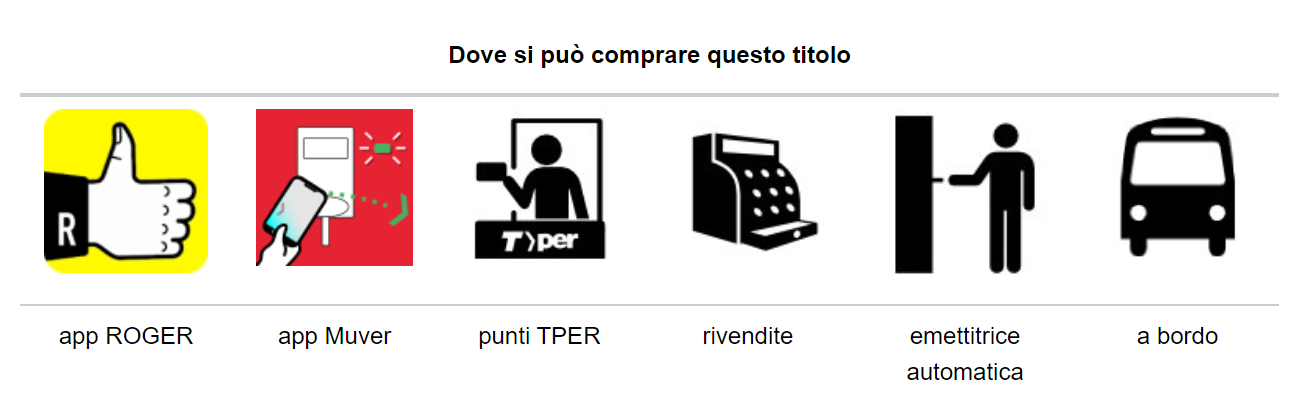
\includegraphics[scale=0.75]{biglietto}

\item  \textbf{十次票 City pass - 10 corse}\\
有效期为 10 次,每次 75 分钟。它允许你在任何路线上在博洛尼亚市区循环,甚至使用多条线路。也可以多人同时使用,每个人都需要打票,一次最多可容纳 7 名乘客。在多人同时使用一张多程票的情况下,必须在三分钟内同时打票,3 分钟后无法再添加乘客。例如,三个人同时使用,需要在3分钟内,连续打票三次。手机APP上买的电子票不支持多人使用。(14欧元/张)
\item  \textbf{日票 Giornaliero}\\
自打票之日起24小时内有效,可用于在博洛尼亚市区内任意路线循环使用,甚至使用多条线路。 它必须在第一次乘车时打票开始计算时间,每次换乘时也需要重新打票。(6欧元/张)

\item  \textbf{年票 Annuale}\\
有效期为一年(从有效期开始算起365天),让你可以每天循环使用,不受行程和时间限制。年票是印有“Mi Muovo”的黄色卡片,其工本费为5欧元,有效期为5年,在Tper销售点出售。如果遗失,补办费用也是5欧元/张。该卡实名制,所以不支持转让使用,每次上车都需要打票。(年票标准价格300欧元/年,另有优惠价格:27岁以下的青年为220欧元/年,70岁以上的老人190欧元/年。博洛尼亚大学为所有就读于本校的学生均提供公交年票的折扣,具体信息请参阅本手册\textbf{7.5.3交通福利 - Tper公交年票}。
\item  \textbf{月票 Mensile}\\
36欧元/月。27岁以下的青年,优惠价格为27欧元/月。每次上车都需要打票。可以在网上购买或者去Tper窗口购买。其有效期为首次打票的日期至当月月底。由于是非记名票,所以可以转让使用,但是不支持多人同时使用(例如不可以两人上车刷两次月票)。
\item  \textbf{使用非接触式卡支付}\\
目前在博洛尼亚、费拉拉和伊莫拉地区的公交车已支持使用非接触式卡在上车时购买车票,票价为1.5欧。使用方法为:上车后在非接触式卡的专用绿色机器上刷卡即可。仅支持非接触式卡,即带有 
\includegraphics[scale=0.6]{carta} 标的预付卡、借记卡和信用卡。如果需要换乘,在换乘时请刷同一张卡,系统将会自动判定。\\
\textbf{注意!}\\
1、绑定在例如Apple Pay和Google Pay等支付软件中的卡和其对应的实体卡将被视为两张不同的卡!\\
2、在遇到查票员时,提供卡号的末尾四位即可。如果是绑定在支付软件中的卡,请提供其设备卡号而非实体卡号的末尾四位。\\
3、使用该方法乘车时,请在上车前通过车辆侧面的标识确认车辆有该刷卡机。首次刷卡购票后,如果你要换乘的车没有该机器或机器故障,则无需再次刷卡,且在75分钟有效期内没有受到处罚的风险。
\item  \textbf{费拉拉(Ferrara)和伊莫拉(Imola)地区的车票价格}\\
\textbf{费拉拉:}次票1.3欧元/张,日票3.5欧元/张,10次票12欧元/张。月票28欧元/张(不可转让给其他人使用),月票32欧元/张(不记名式,可以转让给其他人使用)。年票卡本费5欧元,标准价256欧元/张,优惠价格27岁以下为210欧元/张,70岁以上180欧元/张。\\
\textbf{伊莫拉:}次票1.5欧元/张,10次票14欧元,月票28欧元/张,年票标准价格为256欧元/张,卡片工本费为5欧元/张,优惠价格为27岁以下220欧元/年,70岁以上190欧元/年。


\item  \textbf{机场交通}\\
1、从机场乘坐出租车前往市区\\
根据时间和到达地点的不同,乘车费用可能在15到 25欧元之间波动。\\
2、机场轻轨“马可尼特快”(Marconi Express)\\
在中央车站和机场之间往返,每天从5:40 到 24:00,一年 365 天。单程用时约七分半,单程票11欧元/人,往返票20欧元每人。中央车站的乘坐地点为位于Via de'Carracci的高铁站的中庭内。可以在乘车点购买车票、在官方软件Roger上购买车票、乘车时刷非接触式卡、也可以扫描下方二维码在线购买。\\
\\

\includegraphics[scale=0.4]{marconiqrcode}
%%(https://ticketweb.tper.it/MEXReservation.aspx?lan=IT/)


\end{itemize}


\subsubsection{公交罚款}
\begin{itemize}
\item  75欧,如果5天内交罚款
\item  100欧,标准罚款
\item  300欧,如果因迟迟不交而产生滞纳金后所能累计的最高罚款
\item  6欧,如果乘车没带订阅票(年票、月票),需在5天内持订阅票和身份证件前往Tper服务点缴纳罚款
\end{itemize}
如果你使用的是27欧的青年折扣月票,你还需要在被查票时出示身份证件以证明自己的年龄。\\
如果被罚款,可以向查票员立即支付罚款,或者拿上罚单到Tper窗口支付罚款。如果不当场交罚款,查票人会问你询问护照、居留、税号等个人信息,建议最好当场补交罚款,否则会记录个人诚信档案,对以后在意大利等欧盟国家办理信用卡、找工作造成一些不必要的麻烦。为了不遇到这种情况,大家最好上车打票,不要存在侥幸心理。\\
\\
\textbf{注意!}如果遇到打票机、购票机或非接触式刷卡机故障而造成的无法打票、购票,则可以报告给司机并在遇到查票员时说明情况。建议在遇到此情况时拍摄存留证据。\\
Tper服务点:扫描下方二维码查看\\
\\

\includegraphics[scale=0.3]{tperqrcode}
%%(https://www.tper.it/cliente/i-punti-tper)
\\
\\
\textbf{有关罢工}\\
罢工时,参与罢工的公共交通公司的官网、以及车站站牌上都会公布相关信息,上面能看到本次罢工影响的时间和区域。或者下载诸如“Moovit”等APP,即可收到实时提醒罢工信息和因集会游行而造成的线路改动的通知,也能查询的公交车时间表和实时位置。\\



\section{火车 (Treni)}

\subsection{意大利火车系统介绍}

意大利国铁(Trenitalia)官方网站: trenitalia.it 该网站可以查询火车时刻表、罢工信息、购买火车票等。\\
意大利的火车按速度和行驶范围一般可以分为多个档次:
\begin{itemize}
\item  \textbf{Regionale/Regionale Veloce} 普速列车,相当于国内火车的普快。两种类型的列车速度没有区别,但RV停的站会相对少些。其火车票灵活,类似公交票,乘坐车次和座位可以在上车后灵活选取,纸质票可在票上显示的当天晚上11:59之前使用。每小时的有效期从打票的那一刻开始。上车前必须在站台打票,未来得及打票的,上车后需要及时寻找列车员进行说明,他们会写上时间。\\
车程必须在打票后4小时内结束,特定区域费率规定的例外情况除外。\\
在线购买的车票在所选列车出发后4小时内有效,无需验证。\\
在车票有效期届满时上车的旅客可以继续已经开始的旅程到目的地车站,而无需中途停靠。
\item  \textbf{Intercity(IC) | Intercity Notte} 带有隔间的火车,站点相对少,相当于国内火车的快车。每个车票对应固定车次,固定座位。
\end{itemize}

意大利高铁系统发达,其速度在部分线路(例如博洛尼亚-佛罗伦萨线路)上可以达到300KM/小时以上。高铁列车分为:
\begin{itemize}
\item  \textbf{Frecciarossa(红箭)、Frecciargento(银箭)和Frecciabianca(白箭)}三种,隶属意大利国铁。红箭速度最快,银箭次之,白箭相对最慢。车票对应固定车次,固定座位。红箭和银箭周六有2人行的折扣。
\item  \textbf{Italo} 私人高铁公司,性价比更高。车票对应固定车次,固定座位。
\end{itemize}

\subsection{购票方式}
\begin{itemize}
\item  \textbf{在线购买}\\
在Trenitalia,Italo官方网站购买:\\
https://www.trenitalia.com/\\
https://www.italotreno.it/it\\
官方软件:Trenitalia、Italo等;\\
第三方软件:Omio等;\\
高铁车票提前买折扣很大,如果你早就规划好了行程,建议提早买票。\\
\item  \textbf{线下购买}\\
火车站的自助售票机:\\
售票机一般分为两种,售卖Trenitlia车票的和售卖Italo车票的售票机,请注意区分。支持银行卡/现金支付车票。(机器语言可以选择中文/意大利语/法语/英语等);\\
\\
火车站里的人工柜台:\\
告诉工作人员出发和到达的地点,工作人员会让你选择时间。
但线下购买仅适用于城市市中心大车站,有些小镇的火车站经停站点并没有售票机和人工柜台,只能网上购买车票或者上车时立即向乘务员补票。
\end{itemize}
\textbf{注意:}\\
乘车:
博洛尼亚中央车站Stazione Bologna Centrale有很多站台(地上站台及地下站台,地上站台分为主站台和东、西广场,地下站台则有很多层及停车场),如果是第一次在博洛尼亚中央车站乘车,请至少在发车前30分钟到达车站寻找乘车站台。在火车站乘车,请观看大厅的公告板 (Tabella luminosa) 的出发 (Partenze) 一栏,根据列车编号寻找乘车站台,不要被到达(Arrivi) 的时刻迷惑。在公告板上可以得知要坐的火车是哪个站台,是否晚点 (Ritardo) 。\\
\\
关于车票:
如果购买了Regionale和Regionale Veloce的纸质票,一定要在上车前打票。\\
\\
关于退改票:
高铁的火车票,具体是否可以更改或退款,取决于你购票时所享受的优惠,其退改信息(是否可以退改,退改的时间和手续费等)也会在购票页面写明,请注意查看。\\
\\
关于 Italo 特色车厢:
Italo高铁的Cinema车厢可以看意大利电影,但是需要自备耳机。如果想体验,请在购票时选择Cinema车厢。\\
\\
关于普速列车:如果所去地方仅是途经站,须看站台附近的打印版固定时刻表,黄色为出发,白色为到达。因为公告板 (Tabella luminosa) 主要显示的是起始站和终点站,途径车站滚动显示,不太方便查询。 \\
\\
此外,在Trenitalia官网上注册CartafrecciaYOUNG,如果是30岁以下通常可以享受青年优惠价,并且会时常有邮件推送折扣信息。另外还有学生优惠等,具体信息可查看官网。\\


\section{长途大巴 (Pullman)}
在意大利以及欧洲短途旅行或者长途旅行时,除了火车和飞机以外,还可以选择巴士出行。去同一个城市,坐巴士花的费用往往不到火车费用的一半。但是巴士班次较少,不像火车班次很多。如果是出国或者在意大利境内比较长途的旅行,还可以乘坐夜间巴士,通常是10个小时左右到达目的地,晚上出发,早上就到了,不耽误白天的时间。而且如果打折,有可能买到1欧的廉价票。缺点是在巴士上睡觉不是很舒服。
欧洲巴士系统十分正规且发达,有许多巴士公司供消费者选择,比较著名的有Flixbus、Eurolines、MarinoBus和Itabus等。巴士车票可以在其官网或第三方软件上购买,例如可以用支付宝付款的第三方车票预订软件Omio,综合了意大利很多公司的车票车次信息。
\subsection{购票方式}
以Flixbus为例
\begin{itemize}
\item  \textbf{网站购票:}前往Flixbus官网,选择路线和出发时间后,可以通过信用卡、Paypal、Google pay等多种渠道支付,付款成功后邮箱会收到确认邮件包括车次的具体信息。
\item  \textbf{App购票:}从App Store或Google Play下载FlixBus应用程序。预订车票后使用信用卡付款,付款成功后会收到确认邮件。
\item  \textbf{在销售点购票:}如果更喜欢购买实体车票,可以随时联系销售点预订巴士车票。 也可以前往隶属于Flixbus的旅行社,或前往意大利境内的众多售票处之一。\\
\textbf{以下是一些主要的Flixbus售票处,仅供参考:}\\
Ticketbus Central A - Bus Station, Largo Guido Mazzoni - 罗马\\
Milan Lampugnano Bus Terminal, Via Giulio Natta, 20151 米兰\\
Terminalbus 都灵,Corso Vittorio Emanuele Ii - 都灵\\
Vecchione Agency, Corso Arnaldo Lucci, 24 / Metropark - 那不勒斯\\
ATS S.R.L., Via Giuseppe Capruzzi 224 / C-226 - 巴里\\
Ticketbus Bologna Bus station, Piazza Xx Settembre, 6 - 博洛尼亚\\
Autostazione Trieste,Piazza Liberta '9 – 的里雅斯特\\
\end{itemize}
\textbf{有关其他巴士公司的购票请参阅其官网。}\\
\subsection{乘车地点}
博洛尼亚的乘车地点通常为Autostazione(Piazza XX Settembre 6),但是还请仔细检查购票网站/软件或车票上的说明。

\section{出租车 (Taxi)}
博洛尼亚的出租车主要由C.A.T.联盟运营,24/7全时段提供出租车服务。叫车方式有:\\
致电预约:051 4590\\
短信叫车:发送短信给333 333 0749或336 673 0000,写明乘车地址(街道名称,门牌号),随后会受到系统的回复。\\
使用APP:ItTaxi\\
车费:具体费用表请扫描下方二维码查看。\\
\\

\includegraphics[scale=0.3]{taxiqrcode}\\
%%(https://taxibologna.it/wp-content/uploads/2019/03/TARIFFARIO-ITALIANO.pdf)
\\
付款方式:支持现金、刷卡支付,如果使用ItTaxi叫车,也可以在App上支付。部分出租车也支持支付宝支付,付款码通常在副驾驶座位头枕后,详询出租车司机。


\section{私人租车 (Noleggio auto)}
驾龄超过一年之后才有租车的资格。租车可以在网上申请,然后到租车办事处领车。根据车型和淡旺季,租金40-100多欧/天不等。\\
欧洲流行的租车公司网站有(费用由低到高):
\begin{itemize}
\item https://www.europcar.it
\item http://www.avisautonoleggio.it/default.aspx 
\item https://www.hertz.it/rentacar/reservation/
\end{itemize}


\section{航空 (Aerei)}

\subsection{廉价航空}
在欧洲旅行首推乘坐各家廉价航空公司的航班,如果购票及时很有可能买到超级便宜的机票,而且航线广,欧洲各大城市都有涉及。以下为几家常用链接航空网站:
\begin{itemize}
\item www.ryanair.com
\item www.easyjet.com
\item www.vueling.com
\item www.opodo.it
\end{itemize}

\subsection{关于回国}
打算回国时可能遇到的情况:
\begin{itemize}
\item 第一种情况:第一次申请居留,手里只有居留条,不可以回国,除非签证在有效期内。
\item 第二种情况:持有过期居留,同时有居留条。可以乘坐直飞,不能在欧盟内其他国家转机,可以在俄罗斯、迪拜等转机。
\item 第三种情况:持有有效居留卡,怎么飞都是允许的,包括在申根国,俄罗斯、迪拜、土耳其转机。
\end{itemize}

\section{邮政|通信|网络}

\subsection{邮局常用到的几个业务}
\begin{itemize}
\item 邮政储蓄。可以办理银行卡,和其他银行服务相同。
\item 邮寄业务。挂号信(Raccomandata)是法律性质强的邮寄方法。尤其办理奖学金材料时用到。邮寄前先在窗口领取表格填写,避免延误时间。领取时可以不排队。
\item 居留申请。邮寄居留表格之前,不要忘记购买16欧的印花税。
\item 其他杂务: 水电煤气费用、保险、医药费用等,每张缴费单子(Bolletta)需多缴纳1.3欧的手续费(Commissione),如果在烟草店(Tabacchi)缴费,需多缴纳2欧的手续费。

\end{itemize}

\subsection{快递}
意大利境内主要快递公司包括:DHL、TNT、UPS、FedEx、PosteItaliane 等等。
\begin{itemize}
\item DHL:服务好,送货速度快,但价格更贵。从国内邮寄文件,小物品比较合适,一般3-5个工作日。
\item TNT:意大利最常用的快递公司,价格更便宜,国内EMS包裹到意大利一般也由TNT接管。
\item FedEx: 美国联邦快递,是快递中寄往中国海关税收得最低的公司。
\item PosteItaliane: 意大利邮政,优点是便宜,缺点是时间太慢,不论是在意大利境内的投递还是邮寄回中国都很慢,少则一个月,多则三个月不等。并且在寄回国以后还需要缴纳一定程度的海关税。
\item 人肉快递:价格不定,国内邮寄费用另算。可在学联QQ群、本地微信群内寻找。
\end{itemize}

\subsection{通信}
意大利的国际电话区号是 0039 (+39)。意大利各地区区号都以 0 开头,如米兰 02、罗马 06、博洛尼亚 051 等。所以从中国拨打意大利博洛尼亚市的固定电话的方式为:0039+051+固定电话号码。意大利手机使用的手机网络模式与中国大致相同,所以大部分的中国手机在意大利均可以直接使用。意大利主要的手机运营商有三个,分别是Wind、Tim以及Vodafone,同时也有例如iliad、coop等规模较小的运营商。 \\
办理手机卡的方式为:选择一个运营商,前往其线下店,告诉工作人员要办理新的电话卡,选择你喜欢的套餐,出示护照和税号即可。\\
\\
意大利所有运营商均支持携号转网。选择你想转到的运营商,前往其线下店,告诉工作人员你想转到新的运营商,选择你喜欢的套餐,出示护照和税号即可。工作人员会给你一张新的卡,当你的旧卡无法使用时,新卡就可以使用了,一般在两天左右。\\



手机充值方式一般有三种:
\begin{itemize}
\item 去烟草店(Tabacchi)充值。 
\item 去自己运营商的官方网站充值,可以使用信用卡、Paypal等。 
\item 下载自己运营商的APP,用APP充值,同时也能查看自己的流量剩余,套餐使用情况。
\end{itemize}
打电话回国,中国的国际电话区号为0086,因此从意大利打往中国的电话的拨号方式为:国内固定电话:0086+国内区号(去掉前面的0)+固定电话号码。例如打到天津:0086+22+固定电话号码。国内手机:0086+国内手机号码(不需要在手机号码前加0)。

其他注意事项:意大利全境无漫游费,所以在佩鲁贾或者锡耶纳办理的电话卡在意大利的其他城市也是一样的资费。 
\subsection{网络}

\begin{itemize}
\item 宽带上网:意大利主要网络运营商包括Fastweb、Tim、Infostrada(Wind 公司品牌)及Vodafone等。办理需要带着证件、税号、银行账号、家庭住址等。
\item 户外上网:麦当劳,政府的市政厅或者大学,机场往往都提供免费网络。
\end{itemize}
